\chapter{Crear primer proyecto en Laravel}

A la hora de crear un proyecto en Laravel lo primero que deberíamos hacer es visitar la \href{https://laravel.com/docs/10.x/installation}{documentación}, ya que nos dará distintas opciones dependiendo del sistema operativo en el que nos encontremos. Aparte, podremos ver si ha habido cambios desde la última vez que hayamos creado un proyecto.

\section{Servicios a utilizar}

Antes de crear el proyecto, debemos tomar una serie de decisiones para nuestro \textit{stack} de aplicación. Laravel cuenta con distintos servicios, algunos de ellos necesarios y otros optativos, por lo que deberemos tenerlos en cuenta.

Los servicios entre los que deberemos decidir son:

\begin{itemize}
    \item \textbf{Sistema Gestor de Base de Datos a utilizar}: Laravel permite el uso de distintos sistemas de bases de datos relacionales como son \href{https://dev.mysql.com/downloads/mysql/}{MySQL}, \href{https://www.postgresql.org/}{PostgreSQL} y \href{https://mariadb.org/}{MariaDB}. Por defecto hace uso de \textbf{MySQL}.
    \item \textbf{Sistema de caché}: Podemos hacer uso de distintos sistemas para cachear desde la sesión a información obtenida de la base de datos y también HTML. Por defecto, \textbf{Laravel cachea la sesión en el sistema de ficheros}, pero eso puede ser lento, por lo que se permite hacer uso de sistemas \textbf{clave-valor} para el almacenamiento de información para acelerar el rendimiento de la aplicación web. Se puede elegir \href{https://www.memcached.org/}{Memcached} o \href{https://redis.io/}{Redis} entre otros.
\end{itemize}

Otros servicios que podemos instalar y que nos darán ciertas funcionalidades son:

\begin{itemize}
    \item \textbf{\href{https://github.com/axllent/mailpit}{Mailpit}}: Es un sistema para controlar los emails que envía nuestra aplicación durante el desarrollo. En lugar de enviarlos a las cuentas finales, se quedan almacenados y se pueden visualizar a través de una web que a modo de buzón de correo. También ofrece una API.

    \item Uso de  \href{https://min.io/}{MinIO} para simular el \textbf{almacenamiento en la nube S3}. De esta manera no tendremos que crear un Bucket de pruebas.

    \item Sistema de \textbf{búsqueda \textit{full-text}} en la base de datos gracias a \href{https://laravel.com/docs/10.x/scout#introduction}{Scout} y haciendo uso del backend \href{https://www.meilisearch.com/}{MeiliSearch}.

    \item Creación y automatización de \textbf{tests} utilizando \href{https://www.selenium.dev/}{Selenium}.
\end{itemize}

Estas son algunas de los servicios que podríamos configurar antes de comenzar a crear nuestra aplicación. Para comenzar de manera sencilla nos centraremos únicamente en la elección de la base de datos, dejando el resto de servicios para más adelante.


\section{Instalación mediante Sail y Docker}

En la \href{https://laravel.com/docs/10.x/installation}{documentación} de Laravel nos explica cómo realizar la instalación de distintos modos teniendo en cuenta el sistema operativo, los servicios iniciales que nos interesan y el sistema de instalación que mejor se adapte a nuestro entorno.


El sistema es similar utilizando GNU/Linux, Windows y MacOS, con la salvedad de que en Windows deberíamos instalar Docker Desktop y \textit{Windows Subsystem for Linux} (WSL). De manera generalizada, es necesario tener instalado:

\begin{itemize}
    \item Entorno GNU/Linux
    \item Docker
    \item Docker Compose
    \begin{mycode}{Instalar Docker Compose}{console}{}
ruben@vega:~$ sudo apt install docker-compose
\end{mycode}
\end{itemize}

Para realizar la instalación sólo vamos a elegir tener el servicio de MySQL, para simplificarlo, tal como se ha comentado previamente. Para ello, deberemos ejecutar lo siguiente en el directorio donde nos interese crear el directorio del proyecto.

\begin{mycode}{Usamos el instalador de Laravel}{console}{{\small }}
ruben@vega:~$ curl -s "https://laravel.build/example-app?with=mysql" | bash
\end{mycode}

Este comando lo que va a hacer es descargarse un script que va a ejecutar lo siguiente:
\begin{enumerate}
    \item Se va a asegurar que Docker está corriendo
    \item Va a levantar un contenedor con la imagen “laravelsail/php82-composer” que nos va a crear un directorio llamado \configdir{example-app} con un proyecto limpio de Laravel usando MySQL como SGBD.
    \item Si no tenemos la imagen de MySQL la descarga.
\end{enumerate}


\subsection{Ventajas}

Este sistema de instalación permite realizar un despliegue sencillo en un equipo donde tengamos instalado Docker, con todas las ventajas que ello ofrece, aparte de la posibilidad de elegir los servicios que necesitemos inicialmente.

Podríamos resumir las ventajas en la siguiente lista:

\begin{itemize}
    \item Instalación rápida en un único comando.
    \item Ventajas de usar Docker: todos los desarrolladores usan el mismo contenedor/entorno de desarrollo.
    \item No es necesario tener nada más que Docker instalado en el equipo anfitrión (ni PHP, composer, servicios web, ...).
\end{itemize}

\subsection{Desventajas}
Aunque las ventajas durante el desarrollo de aplicaciones son notables, también pueden existir algunas desventajas:

\begin{itemize}
    \item El servidor web que se arranca por defecto no es el más recomendado para despliegues en producción, obteniendo mejor rendimiento con el servidor web \href{https://nginx.org/en/}{Nginx}.

    \item En un principio puede resultar “raro” desarrollar dentro de un contenedor.
\end{itemize}


\section{Iniciar servicios}

Una vez terminada la descarga del código y tras realizar las acciones que necesita, el propio asistente nos avisa de qué tenemos que realizar para que nuestro entorno arranque.

\begin{mycode}{Arrancamos los servicios}{console}{}
ruben@vega:~$ cd example-app && ./vendor/bin/sail up -d
[+] Running 2/2
  Container example-app-mysql-1         Started    0.4s
  Container example-app-laravel.test-1  Started    0.7s
\end{mycode}

Y con ello podemos ir al puerto 80 a través de nuestro navegador y veremos la página principal para comprobar que todo ha ido bien.

\begin{center}
    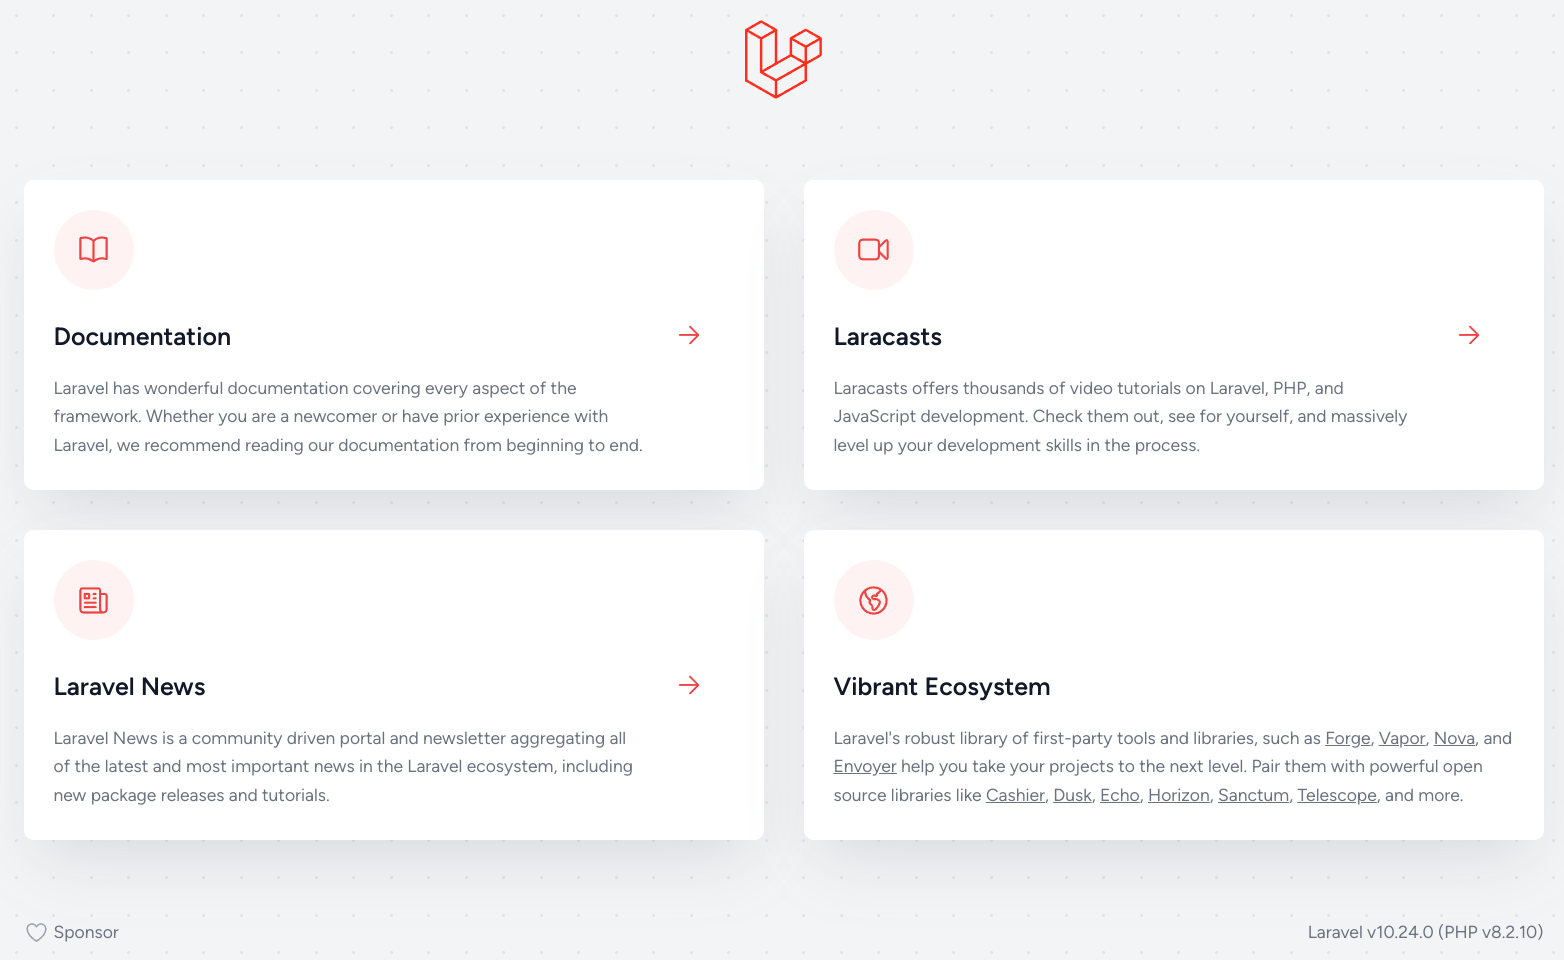
\includegraphics[frame,width=0.7\linewidth]{intro.png}
\end{center}


\chapter{Variables de entorno}
Todo proyecto de Laravel cuenta con unas variables de entorno del proyecto. Es un fichero de configuración situado en la raíz del proyecto que se llama \configfile{.env} y en él se encuentran las credenciales para acceder a la base de datos, servidor SMTP, ...

Dado que hemos generado el entorno a través del asistente, se ha rellenado con la configuración por defecto, entre las que nos encontramos que la aplicación tiene \textbf{el modo debug activado}. Durante el desarrollo nos va a ayudar para poder hacer \textit{debugging} mientras realizamos acciones, pero esta opción debería estar deshabilitada al poner la aplicación en producción.

Por último, es conveniente recordar que este fichero \textbf{nunca debería estar en un repositorio público}, ya que contiene información sensible como lo son los credenciales de acceso a bases de datos o servicios externos.

\errorbox{\textbf{Cuidado con versionar el fichero “\texttt{.env}”, ya que contiene información sensible}}